\documentclass[letterpaper,11pt]{report}
% Change margins to 1 inch on all sides
\addtolength{\oddsidemargin}{-.875in}
\addtolength{\evensidemargin}{-.875in}
\addtolength{\textwidth}{1.75in}
\addtolength{\topmargin}{-.875in}
\addtolength{\textheight}{1.75in}
\usepackage{float}
\usepackage{graphicx}
\usepackage{footnote}
\usepackage{longtable}
\usepackage{multirow}
\usepackage{tablefootnote}
\usepackage{tabularx}
\usepackage{url}
\DeclareGraphicsExtensions{.pdf,.png,.jpg}

%%%%%%%%%%Start of report
\begin{document} 
\begin{savenotes}
\pagestyle{plain}
\title{CS896 Introduction to Web Science\\Fall 2013\\Report for Assignment 2}
\author{Corren G. McCoy}
 
\date{September 19, 2013}
\maketitle

\renewcommand*\thesection{\arabic{section}}
\setcounter{section}{0}

\setcounter{tocdepth}{4}
\tableofcontents
 \listoffigures
 \listoftables
\newpage


%%%%%%%%%%Chapter Exercises
\section{Question 1}
\subsection{Problem}Write a Python program that extracts 1000 unique links from Twitter.
\subsection{Response}We used Twitter's Search API (\url{https://dev.twitter.com/docs/api/1.1}) to search for recent tweets which contained any of the following keywords: ``Putin'', ``Syria'', ``Assad'', ``Obama,'' or ``chemical weapons''. Our Python program, \emph{ExtractLinks}, as shown in Appendix \ref{chap:Python Source - Extract Links}, stores the keywords in a list object with each element passed individually to the API as part of the query string. The text of each tweet returned from the search was parsed to remove any URLs which were then written to a text file (i.e., tweetFileCandidates.txt). Using the keywords indicated, we built a collection of approximately 8400 candidate URLs from which we sought to obtain the desired 1000 unique links. The unique links were identified using line-by-line processing of the tweetFileCandidates list. Each shortened URL was opened in order to verify the reference to an existing web site. Any URL with a response status of 200 was checked against the a master domain list. The full URL was obtained from the response header. To ensure uniqueness only one URL from any domain was allowed. This was facilitated by storing the domain as the key and the full URL as the value in a dictionary object which inherently ensures a unique domain for each key. Processing of the URLs in the tweetFileCandidates was terminated once 1000 domain URLs were obtained. This final list was then printed to a text (i.e., tweetFile1000.txt). A sample of the URLs harvested from Twitter is shown in Table \ref{tab:SampleTwitterURLs}.

\begin{table}[htbp]
	\centering
    \begin{tabular}{l}
		\hline
    \url{http://investmentwatchblog.com/ }       \\ \hline
    \url{http://whithererehwon.wordpress.com/}   \\ \hline
    \url{http://maxcouti.blogspot.com/}          \\ \hline
    \url{http://kevskewl.wordpress.com/}         \\ \hline
    \url{http://www.marketing-projects.biz/}     \\ \hline
    \url{http://mundonovovelho.blogspot.com.br/} \\ \hline
    \end{tabular}
		\caption{Sample Twitter URLs}
		\label{tab:SampleTwitterURLs}
\end{table}


%%%%%%%%%%Chapter Exercises
\section{Question 2}
\subsection{Problem}Download the TimeMaps for each of the target URIs. Create a histogram of URIs versus number of Mementos (as computed from the TimeMaps).
\subsection{Response}Using our list of 1000 Twitter URIS, we used the ODU Memento Aggregator to generate the associated TimeMaps using our Python program \emph{getTimeMaps} which is described in Appendix \ref{chap:Python Source - Get TimeMaps}. A sample from the TimeMap output is shown in Table \ref{tab:SampleTimeMapOutput}. The Rel-Tag\footnote{\url{http://www.microformats.org/wiki/Rel-Tag}} of each TimeMap was examined to determine whether the information presented was tagged as a memento.  We specifically looked for valid combinations of either ''first memento'', ''last memento'', ''memento first'', ''memento last'', or ''first last memento'' using regular expressions in Python. Each occurence of a memento tag increased the counter for each URI. The URI and the associated memento count were saved to a comma-delimited text file (i.e., histogram.txt) that was used as the data source for our histogram. We used the graphing functions in R to produce the histogram shown in Figure \ref{fig:mementoHistogram}. The histogram is representative of the long tail\footnote{\url{http://en.wikipedia.org/wiki/The_Long_Tail}} with over 96\% of the URIs having less than 2,500 mementos with a much sparser distribution in the range of 2,500 to approximately 30,000.

\begin{table}[htbp]
\centering
    \begin{tabular}{l}
		\hline
\url{<http://http://mementoproxy.cs.odu.edu/aggr/timemap/link/http://investmentwatchblog.com/>; rel="self";type="application/link-format", }\\ \hline
 \url{<http://mementoproxy.cs.odu.edu/aggr/timegate/http://investmentwatchblog.com/>; rel="timegate",<http://investmentwatchblog.com/>;rel="original",} \\ \hline
 \url{<http://web.archive.org/web/20100212220649/http://investmentwatchblog.com/>; rel="first memento";datetime="Fri, 12 Feb 2010 22:06:49 GMT",}  \\ \hline
 \url{<http://web.archive.org/web/20100409065504/http://investmentwatchblog.com/>; rel="memento";datetime="Fri, 09 Apr 2010 06:55:04 GMT",}  \\ \hline
 \url{<http://web.archive.org/web/20100415152016/http://investmentwatchblog.com/?>; rel="memento";datetime="Thu, 15 Apr 2010 15:20:16 GMT",} \\ \hline
    \end{tabular}
		\caption{Sample TimeMap Output}
		\label{tab:SampleTimeMapOutput}

\end{table}

\begin{figure}[htbp]
	\centering
		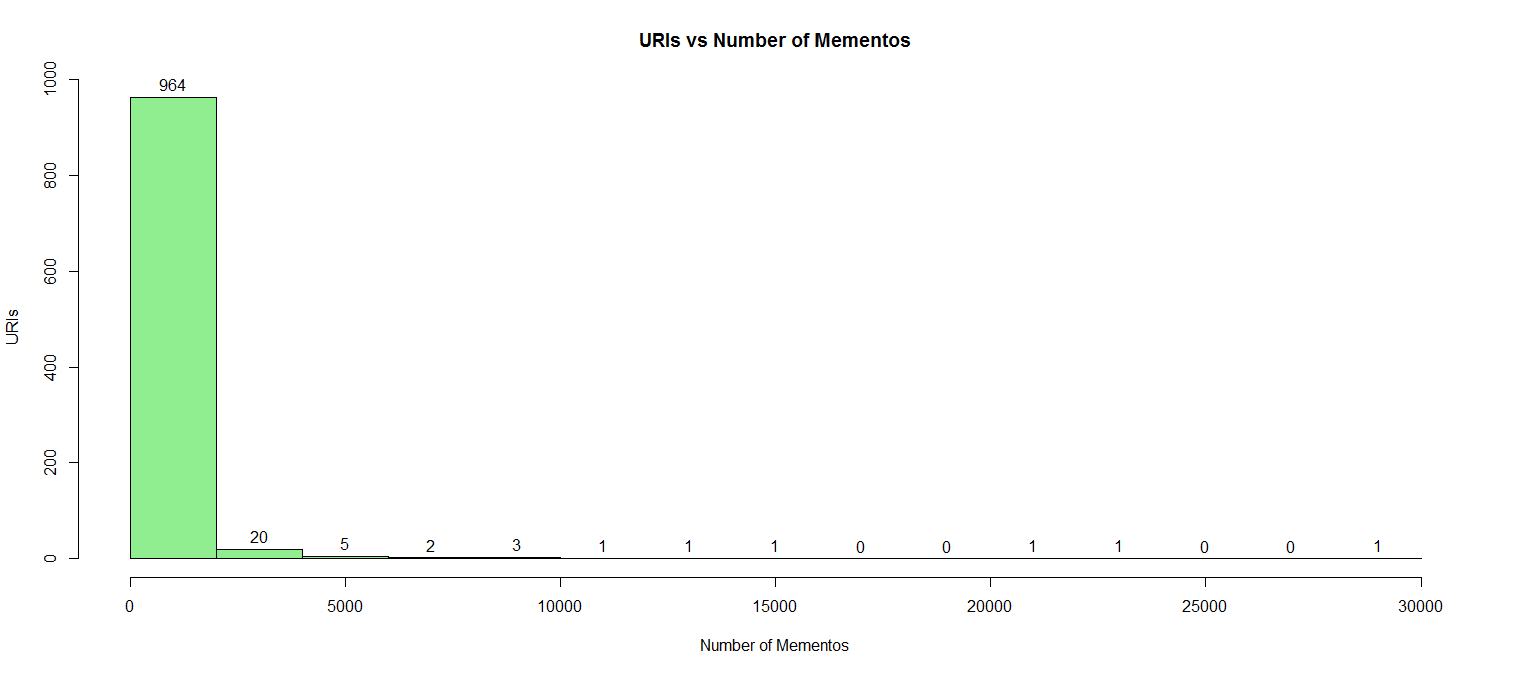
\includegraphics[width=1.00\textwidth]{mementoHistogram.png}
	\caption{URIs vs. Mementos}
	\label{fig:mementoHistogram}
\end{figure}


%%%%%%%%%%Chapter Exercises
\section{Question 3}
\subsection{Problem}Estimate the age of each of the 1000 URIs using the ''Carbon Date'' tool. For URIs that have at least one memento and an estimated creation date, create a graph with age (in days) on one axis and number of mementos on the other
\subsection{Response}


\end{savenotes}

% produce the bibliography for the citations in your paper.
\bibliographystyle{abbrv}
\bibliography{cmccoy}

\appendix
\addcontentsline{toc}{chapter}{Appendices}

%%Appendix A
\chapter{Python Source for extractLinks.py} \label{chap:Python Source - Extract Links}
\input{extractLinks.py}
\chapter{Python Source for getTimeMaps.py} \label{chap:Python Source - Get TimeMaps}
\input{getTimeMaps.py}
\chapter{R Source for Histogram} \label{chap:R Source - Histogram}
\input{histogram.r}


\end{document} 
%%%%%%%%%%Ed of report
